\documentclass[../main.tex]{subfile}
\graphicspath{{\subfix{../images}}}
\begin{document}

我们的物体检测系统由三个模块组成。第一个模块产生独立于类别的候选区域。这些候选定义了可供我们的检测器使用的候选检测的集合。第二个模块是一个从每个区域提取一个固定长度的特征向量的大型卷积神经网络。第三个模块是一组类别特定的线性SVM。在本节中,我们将介绍我们对每个模块的设计决定,描述它们在测试时的使用情况,详细说明它们的参数是如何习得的,并展示在PASCAL VOC 2010-12和ILSVRC2013上的检测结果。

\subsection{模块设计}

\paragraph{区域候选。}最近的论文提供了各种生成与类别无关的区域候选的方法。例子包括:objectness[1]、selective search[39]、category-independent object proposals[14]、constrained parametric min-cuts(CPMC)[5]、multi-scale combinatorial grouping[3]和Cires¸an等人[6]通过将CNN应用于规则间隔的方形作物,检测有丝分裂细胞,这是区域建议的一个特殊案例。虽然R-CNN与特定的区域提议方法无关,但我们使用选择性搜索,以便与先前的检测工作(例如,[39,41])进行控制变量比较。

\paragraph{特征提取。}我们使用Krizhevsky等人\cite{alexnet}描述的CNN的Caffe\cite{caffe}实现,从每个候选区域中提取4096维的特征向量。特征的计算通过将减去均值的227×227RGB图像通过五个卷积层和两个全连接层进行前向传播。关于更多的网络结构细节,我们请读者参考\cite{alexnet, caffe}。

\begin{figure}[htb]
    \centering
    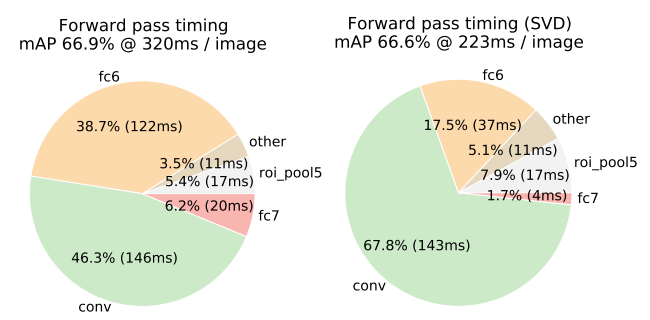
\includegraphics[width=\textwidth]{fig2.png}
    \caption{来自VOC 2007训练集中的\textbf{扭曲训练样本}。}
    \label{fig:fig2}
\end{figure}

% NOTE 有一句话并不清楚
为了计算一个候选区域的特征,我们必须首先将该区域的图像数据转换为与CNN兼容的格式(其架构要求输入大小为固定的$227 \times 227$像素)。在对于任意形状区域的许多可能的转换中,我们选择了最简单的。无论候选区域的大小或长宽比如何,我们都会将其周围的紧缩边界框中的所有像素扭曲到所需的大小。在变形之前,我们扩张紧缩边界框,以便在变形的尺寸下,原始框周围正好有$p$个像素的变形图像背景(我们使用$p=16$)。图\ref{fig:fig2}显示了一个随机抽样的被包裹的训练区域。附录\ref{app:transformation}中讨论了可替代的扭曲方法。

\subsection{检测的测试阶段}

在测试时间,我们对测试图像进行选择性搜索,以提取大约2000个候选区域(我们在所有实验中使用选择性搜索的 "快速模式")。我们对每个候选进行扭曲,并通过CNN进行前向传播,以计算出特征。然后,对于每个类别,我们使用为该类别训练的SVM对每个提取的特征向量进行评分。得到图像中的所有被打分的区域后,我们使用一个贪婪的非最大抑制(对每个类别独立),如果一个区域与一个更高得分的选定区域的交叉重叠(IoU)大于习得的阈值,则拒绝该区域。

\paragraph{运行分析。}有两个特性使检测变得高效。首先,所有的CNN参数在所有类别中都是共享的。第二,与其他常见的方法相比,CNN计算的特征向量是低维的,如带有视觉词包编码的空间金字塔。例如,UVA检测系统[39]中使用的特征比我们的大两个数量级(360k vs. 4k-维)。

这种共享的结果是,计算区域候选和特征的时间(GPU上的13s/图像或CPU上的53s/图像)被所有类别分摊。唯一针对类的计算是特征和SVM权重之间的点乘和非最大抑制。在实践中,一个图像的所有点积都被打包成一个单一的矩阵-矩阵乘积。特征矩阵通常为2000×4096,SVM权重矩阵为4096×N,其中N为类的数量。

这一分析表明,R-CNN可以在不借助近似的技术,如散列,的情况下扩展到成千上万的类别。即使有10万个类,所产生的矩阵乘法在现代多核CPU上只需要10秒。这种效率不仅仅是使用区域候选和共享特征的结果。UVA系统,由于其高维特征,会慢两个数量级,同时需要134GB的内存来存储10万个线性预测器,而我们的低维特征只需要1.5GB。

将R-CNN与Dean等人[8]最近关于使用DPM和散列的可扩展检测工作进行对比也很有意思。他们报告说,在引入10k个干扰物类别时,VOC 2007的mAP约为16\%,每幅图像的运行时间为5分钟。使用我们的方法,10k个检测器可以在CPU上运行约1分钟,而且由于没有进行近似,mAP将保持在59\%(3.2节)。

\subsection{训练}

\paragraph{监督预训练。}我们在一个大型的辅助数据集(ILSVRC2012分类)上对CNN进行判别性预训练,只使用图像级别的注释(该数据没有边界框标签)。预训练是使用开源的Caffe CNN库\cite{caffe}进行的。简而言之,我们的CNN几乎达到了与Krizhevsky等人\cite{alexnet}相匹配的性能,在ILSVRC2012分类验证集上的top-1错误率比之高2.2\%。这种差异训练过程简化造成的。

\paragraph{特定领域微调。}为了使我们的CNN适应新的任务(检测)和新的领域(扭曲的候选窗口),我们仅使用扭曲的区域候选来继续对CNN参数进行随机梯度下降(SGD)训练。除了用一个随机初始化的(N+1)分类层(其中N是物体类别的数量,加上1是背景)取代CNN的ImageNet特定的1000路分类层外,CNN的架构没有变化。对于VOC,$N=20$,对于ILSVRC2013,$N=200$。我们将所有与ground-truth框重叠$\geq 0.5$的区域候选作为该框类别的正例,其余的作为负例。我们以0.001的学习率(初始预训练率的1/10)开始SGD,这允许微调在不使初始化失效的情况下取得进展。在SGD的每次迭代中,我们均匀地对32个正例窗口(所有类别)和96个背景窗口进行采样,以构建一个128大小的迷你批。我们之所以偏向于对正例窗口进行抽样,是因为与背景相比,正例窗口是非常罕见的。

\paragraph{物体类别分类器。}考虑训练一个检测汽车的二分类器。很明显,一个紧密包围着汽车的图像区域应该是一个正例。同样,很明显,一个与汽车无关的背景区域应该是一个负例。不太清晰的是如何标记一个与汽车部分重叠的区域。我们用IoU重叠阈值来解决这个问题,低于这个阈值的区域被定义为负例。重叠阈值,0.3,是通过在验证集上对$\left\{ 0, 0.1, \ldots, 0.5 \right\}$进行网格搜索得到的。我们发现,精心选择这个阈值是很重要的。如同在[39]中,将其设置为0.5,使mAP减少了5个点。同样地,将其设置为0会使mAP减少4个点。正例被简单地定义为每个类别的ground-truth边界框。

一旦提取了特征并应用了训练标签,我们就为每个类别优化一个线性SVM。由于训练数据太大,无法装入内存,我们采用了标准的难负例挖掘方法[17, 37]。难负例挖掘方法收敛很快,在实践中,mAP仅在对所有图像进行一次处理后就不再增加。

在附录\ref{app:posi_neg}中,我们讨论了为什么在微调与SVM训练中对正负样本的定义是不同的。我们还讨论了训练检测SVM所涉及的权衡,而不是简单地使用微调CNN最后的softmax层的输出。

\subsection{在PASCAL VOC 2010-12上的结果}

按照PASCAL VOC的最佳实践[15],我们在VOC 2007数据集上验证了所有的设计决策和超参数(3.2节)。对于VOC 2010-12数据集的最终结果,我们在VOC 2012 train上对CNN进行了微调,并在VOC 2012 trainval上优化了我们的检测SVMs。对于两种主要的算法变体(有边界盒回归和无边界盒回归),我们只向评估服务器提交了一次测试结果。

表1显示了VOC 2010上的完整结果。我们将我们的方法与四个强大的基线进行比较,包括SegDPM[18],它将DPM检测器与语义分割系统[4]的输出结合起来,并使用额外的检测器之间的背景和图像分类器的重新评分。最有意义的是与Uijlings等人[39]的UVA系统的比较,因为它与我们的系统使用了相同的区域候选算法。为了对区域进行分类,他们的方法建立了一个四级空间金字塔,并用密集采样的SIFT、Extended OpponentSIFT和RGBSIFT描述符填充它,每个向量用4000字的编码簿量化。分类是用直方图相交核SVM进行的。与他们的多特征、非线性核SVM方法相比,我们在mAP方面取得了很大的改进——从35.1\%到53.7\%的mAP,同时速度也更快(\ref{sec:ablation}节)。我们的方法在VOC 2011/12测试中取得了类似的性能(53.3\% mAP)。

\subsection{在ILSVRC2013检测上的结果}

我们使用了与PASCAL VOC相同的系统超参数,在200类ILSVRC2013检测数据集上运行R-CNN。我们遵循同样的协议,向ILSVRC2013评估服务器只提交了两次测试结果,一次有边界框回归,一次没有。

\begin{figure}[htb]
    \centering
    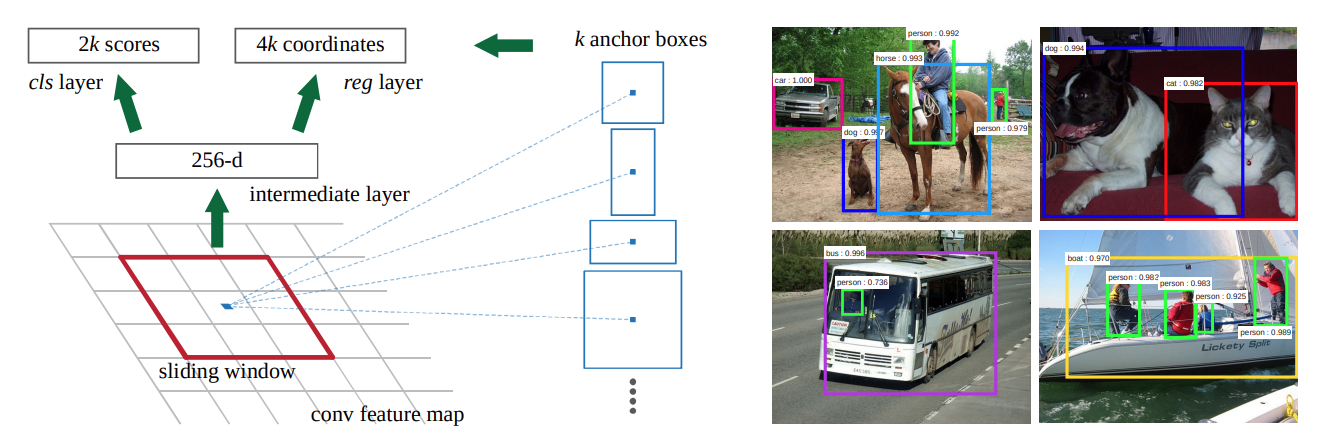
\includegraphics[width=\textwidth]{fig3.png}
    \caption{\textbf{(左) ILSVRC2013检测测试集的平均精度。}前面带*的方法表示使用了外部训练数据 (在所有情况下,图像和标签来自ILSVRC分类数据集)。\textbf{(右) 每个方法的200个平均精度值的箱形图。}没有显示OverFeat赛后结果的箱形图,因为还没有可用的每类的AP(R-CNN的每类AP见表8。R-CNN的每级AP在表8中,也包括在上传到arXiv.org的技术报告源中;见R-CNN-ILSVRC2013-APs.txt)。红色的线标志着AP的中位数,方框底部和顶部是第25和75个比例。胡须延伸至每种方法的最小和最大AP。每个AP在晶须上被绘制成一个绿色的点(最好用数字放大查看)。}
    \label{fig:fig3}
\end{figure}

图\ref{fig:fig3}将R-CNN与ILSVRC2013比赛中的参赛模型以及OverFeat\cite{overfeat}的赛后结果进行了比较。R-CNN实现了31.4\%的mAP,明显领先于OverFeat的第二好成绩24.3\%。为了让大家了解AP在不同类别中的分布情况,我们还展示了箱形图,并在文末的表8中列出了每类AP的表格。大多数竞争者(OverFeat、NEC-MU、UvAEuvision、Toronto A和UIUC-IFP)都使用了卷积神经网络,这表明在将CNN应用于物体检测的细微差别将导致结果的大不相同。

在第4节中,我们概述了ILSVRC2013检测数据集,并提供了我们在其上运行R-CNN时所作选择的细节。

\end{document}

